\documentclass{article}
\usepackage{hyperref}
\usepackage{amsmath}
\usepackage{amssymb}
\usepackage{pgfplots}
\usepackage{float}
\usepackage{todonotes}
\usepackage{tikz}
\usepackage[shortlabels]{enumitem}

\renewcommand{\Re}{\mathbb{R}}
\newcommand{\Li}{\mathcal{L}}
\newcommand{\Ex}{\mathbb{E}}
\renewcommand{\Pr}{\mathbb{P}}
\newcommand{\Hy}{\mathcal{H}}
\newcommand{\sign}{\text{sign}}
\newcommand{\error}{\text{error}}

\newcommand\bigO[1]{
    \ensuremath{\mathcal{O}\left(#1\right)}
    }

\newcommand{\sigmoidPlot}{
    
    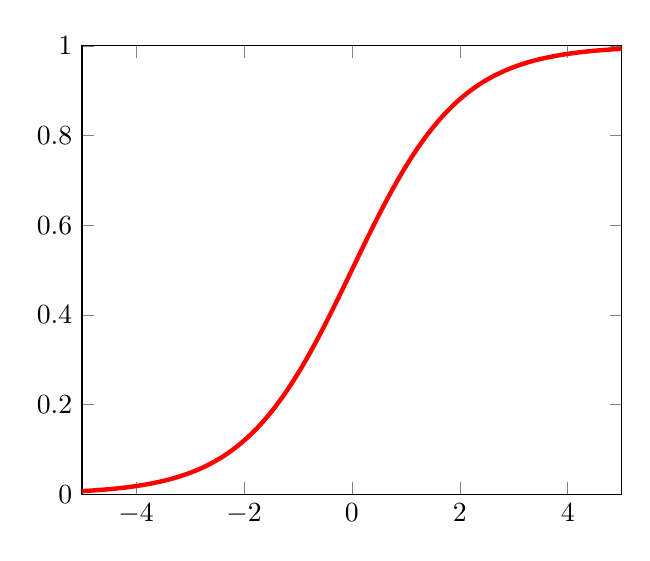
\begin{tikzpicture}
        \begin{axis}[xmin=-5, xmax=5, ymin=0, ymax=1, samples=150]
        \addplot[red, ultra thick] {1/(1+exp(-x))};
        \end{axis}
    \end{tikzpicture}
    
    }

\usetikzlibrary{positioning, calc}
\usetikzlibrary{arrows.meta}

\tikzstyle{circlebox}=[circle,thick,draw=black!75,minimum size=8mm]
\tikzstyle{inputnode}=[circlebox, draw=blue!75]
\tikzstyle{hiddennode}=[circlebox, draw=orange!75]
\tikzstyle{outputnode}=[circlebox, draw=orange!75]
\tikzstyle{simplebox}=[rectangle,thick,draw=black!75,
fill=black!20,minimum size=4mm]
\tikzstyle{textbox}=[rectangle,thick,minimum size=4mm,draw=black!0,
fill=black!0]
\tikzstyle{halfvdistance}=[yshift=-0.7cm]
\tikzstyle{abovebetween}=[xshift=-2.7mm]
\tikzstyle{edgepath} = [-Latex,->,shorten >=1pt,-stealth,semithick, rounded 
corners=5pt]

\def \nodedv {0.735cm}
\def \nodedh {0.65cm}

\tikzset{
    between/.style args={#1 and #2}{
        at = ($(#1)!0.5!(#2)$)
    }
}

\begin{document}
    \section{Subjects}
    \begin{itemize}
        \item Representation based
        \item Density based
        \item Subspace
    \end{itemize}
    
    \section{Notes}
    
    \subsection{Representation based}
    Here are some of the main algorithms within representation based clustering:
    \begin{itemize}
        \item $K$-Means
        \item $K$-Medoids
        \todo{Any more?}
    \end{itemize}
    Common for all of these algorithms, is that they all use some point which 
    summarizes or ``represents'' the cluster, a common choice being the mean 
    (or the \textit{centroid}) $\mu_i$. If we were to make this partitioning in 
    an exhaustive way, we would simply find all possible partitions (i.e. all 
    possible means) and pick the best. Doing this brute-force approach, results 
    in \bigO{k^n/k!} clusterings of $n$ points into $k$ groups, so this is not 
    practically feasible at all. Let's instead look at some smarter algorithms 
    for solving this problem.
    
    \subsubsection{$K$-Means}
    The idea of $k$-means is for some $k$ to form $k$ groups so that the sum of 
    the (squared) distances between the mean of the groups and their elements 
    is minimal. In other words we want to minimize the squared error measure as 
    we often do for linear regression.
    
    Given that our points $p_i=(p_{i1},\dots,p_{id})$ are a point in a 
    $d$-dimensional vector space, where the mean of a set of points is defined 
    (e.g. euclidean). We then have that the centroid $\mu_C$ for some cluster 
    $C$ is defined as:
    \begin{equation*}
        \mu_C = \frac{1}{|C|} \sum_{p_i\in C}p_i
    \end{equation*}
    We can then compute the \textit{sum of squared errors} as:
    \begin{equation*}
        SSE(C)=\sum_{i=1}^{k}\sum_{x_j\in C_i}\|x_j-\mu_i\|^2
    \end{equation*}
    We then want to find the clustering that minimizes SSE:
    \begin{equation*}
        C^*=\arg\min_C SSE(C)
    \end{equation*}
    We can outline the $k$-means algorithm as:
    \begin{enumerate}
        \item Partition the objects into $k$ non-empty subsets
        \item Compute the centroids of the clusters of the current partition. 
        The centroid is the center (mean point) of the cluster.
        \item Assign each object to the cluster with the nearest representative.
        \item Go back to Step 2, stop when representatives do not change.
    \end{enumerate}
    Which gives us the following pseudocode:
    \begin{algorithm}
        \caption{$k$-means}\label{alg:k-means}
        \begin{algorithmic}
            \Procedure{$k$-means}{$D,k,\epsilon$}\Comment{asd}
            \State $t \gets 0$
            \State Randomly initialize $k$ centroids 
            $\mu_{t1},\mu_{t2},\dots,\mu_{tk} \in \Re^d$
            \Repeat
                \State $t \gets t+1$
                \State $C_j \gets \emptyset$ for all $j = 1,\dots,k$
                \State \textit{// Cluster assignment step}
                \ForAll{$x_j\in D$}
                    \State $j^* \gets \arg\min\limits_{i=1,\dots,k} \|x_j - 
                    \mu_{ti}\|^2$
                    \Comment{\textit{Assign $x_j$ to closest centroid}}
                    \State $C_{j^*} \gets C_{j^*} \cup \{x_j\}$
                \EndFor
                \State \textit{// Centroid Update Step}
                \ForAll{$i=1$ to $k$}
                    \State $\mu_{ti} \gets \frac{1}{|C_i|}\sum_{x_j \in C_i} 
                    x_j$
                \EndFor
            \Until{$\sum_{i=1}^{k}\|\mu_{ti}-\mu_{t-1,i}\|^2 \leq \epsilon$}
            \EndProcedure
        \end{algorithmic}
    \end{algorithm}
    Then, if we are using euclidean distance (the manhattan distance could look 
    differently), the voronoi diagram (a visual representation of the clusters) 
    will look like this image:\\
    
    \voronoi{4}{2}\\
    
    \textbf{Strengths}
    \begin{itemize}
        \item Relatively efficient \bigO{tkn} where $n$ is \#objects, $k$ is 
        \#clusters and $t$ is \#iterations
        \item Normally $k$ and $t$ are both much smaller than $n$ so in 
        practice it's only $n$ that matters.
        \item It's easy to implement
    \end{itemize}
    \textbf{Weaknesses}
    \begin{itemize}
        \item Applicable only in vector spaces where the mean is defined
        \item We need to specify the number of clusters $k$ in advanced (it's a 
        hyper-parameter)
        \item It's sensitive to noisy data and outliers
        \item Clusters are forced to have convex shapes, for example here is a 
        voronois diagram with many clusters:\\
        \voronoi{30}{4}
        \item Both results and running time are very dependent on the initial 
        selection of $k$-means, as it often terminates at a \textit{local 
        optimum}, however there do exist methods for good initialization.
    \end{itemize}
    There are several variant of $k$-means, e.g. ISODATA which extends 
    $k$-means by merging and splitting clusters to eliminate very small 
    clusters, at a cost of more hyper-parameters.
    
    \subsubsection{$K$-Medoids}
    $k$-means implicitly assume euclidean distance, since we need to minimize 
    the distance to the mean, there are variations for other distance functions.
    
    The $k$-medoid algorithm is more general, it's motivated by the $L_1$ norm 
    (Manhattan) distance and also works in spaces where a mean is not defined. 
    We just need to be able to compute pairwise distances. Furthermore 
    $k$-medoid will turn out to be more robust to noise. The general $L_p$ 
    distance metric (Minkowski-Distance) is defined as:
    \begin{equation*}
        d_p(x,y)=\sqrt[p]{\sum_{i=1}^{d}|x_i-y_i|^p}
    \end{equation*}
    Where Euclidean is the $L_2$ metric and Manhattan is the $L_1$ metric.
    Other examples of distance functions is the maximum metric:
    \begin{equation*}
        d_\infty(x,y)=\max_{1\leq i\leq d} |x_i-y_i|
    \end{equation*}
    Or for two sets we could define it as:
    \begin{equation*}
        d_{set}(x,y)=\frac{|x\cup y| - |x\cap y|}{|x\cup y|}
    \end{equation*}
    Or we could use the Hamming distance etc.
    
    Now for the basic idea of $k$-medoid, we start by defining some notions. 
    First of all, the medoid $m_C$ is the representative object for a cluster 
    $C$. The compactness of a clustering $C$ is measured as:
    \begin{equation*}
        TD=\sum_{i=1}^{k}\sum_{p\in C}\dist(p, m_C)
    \end{equation*}
    We can then comput the $k$-medoids, using PAM as follows:
    \begin{enumerate}
        \item Select $k$ objects arbitrarily as medoids, then assign each 
        remaining (non-medoid) object to the cluster with the nearest 
        representative. We will then compute the $TD$ and name it $TD_{current}$
        \item For each pair (medoid $M$, non-medoid $N$), exhaustively compute 
        the $TD$ value for the partition if $N$ was the medoid instead of $M$, 
        $TD_{NM}$.
        \item Select the non-medoid $N$ for which the $TD_{NM}$ value was 
        minimal, if the $TD$ value is smaller than $TD_{current}$ then:
        \begin{enumerate}
            \item Swap $N$ with $M$
            \item Set $TD_{current} \gets TD_{NM}$
            \item Go back to Step 2
        \end{enumerate}
        \item Stop
    \end{enumerate}
    
    \textbf{Strength}
    \begin{itemize}
        \item We can use it on arbitrary objects (e.g. points or sets) and 
        arbitrary distance measures
        \item Not quite as sensitive to noisy data and outliers as $k$-means
    \end{itemize}
    \textbf{Weaknesses}
    \begin{itemize}
        \item Inefficient
        \item We need to specify number of clusters $k$ in advance and clusters 
        need to have convex shapes
    \end{itemize}
    
    \subsubsection{Expectation Maximization (EM)}
    In $k$-means, each point could only belong to precisely one cluster, EM is 
    soft-assignment of points to clusters, so each point has a probability of 
    belonging to each cluster. We represent a cluster by a probability 
    distribution, usually we will represent it as center point $\mu_C$ and a 
    $d\times d$ covariance matrix $\Sigma_C$ for the points in the cluster $C$. 
    If we assume that the each cluster $C_i$ is characterized by a multivariate 
    normal distribution, then we can define the density function for cluster 
    $C$ as:
    \begin{equation*}
        P(x|C)=\frac{1}{\sqrt{(2\pi)^d|\Sigma_C|}} \cdot 
        e^{-\frac{1}{2}(x-\mu_C)^T \cdot (\Sigma_C)^{-1} \cdot (x-\mu_C)}
    \end{equation*}
    We can then estimate the a-priori probability of class $C_i$, $P(C_i)$ as 
    the relative frequency $W_i$. I.e. we define the $P(C_i)$ as the fraction 
    of contribution from the entire data-set $D$ to class $C_i$:
    \begin{equation*}
        P(x)=\sum_{i=1}^{k}W_i \cdot P(x|C_i)
    \end{equation*}
    We can then compute the probability that $x$ belongs to cluster $C_i$ as:
    \begin{equation*}
        P(C_i|x)=W_i \cdot \frac{P(x|C_i)}{P(x)}
    \end{equation*}
    Now, we can compute a measure of the quality of a clustering $M$ as $E(M)$ 
    which indicates the probability that the data $D$ has been generated by the 
    distribution model $M$:
    \begin{equation*}
        E(M)=\sum_{x\in D} \log(P(x))
    \end{equation*}
    Which is what we will try to maximize in EM. Which brings us to our 
    algorithm:
    \begin{algorithm}
        \caption{Expectation Maximization}\label{alg:EM}
        \begin{algorithmic}
            \Procedure{EM}{$D,k$}
                \State Generate an initial model $M'=(C_1',\dots,C_k')$
                \Repeat
                    \State \textit{// (Re-) assign points to clusters - 
                    expectation step}
                    \ForAll{$x \in D$}
                        \ForAll{$C_i,\, i=1,\dots,k$}
                            \State Compute $P(x|C_i)$, $P(x)$ and $P(C_i|x)$
                        \EndFor
                    \EndFor
                    \State \textit{// (Re-) compute the model - maximization 
                    step}
                    \ForAll{$C_i,\, i=1,\dots,k$}
                        \State Recompute $W_i$, $\mu_C$ and $\Sigma_C$
                        \State Compute a new model $M=\{C_1,\dots,C_k\}$ using 
                        $W_i$, $\mu_C$ and $\Sigma_C$
                        \State Replace $M'$ with $M$
                    \EndFor
                \Until{$|E(M)-E(M')| < \epsilon$}
            \EndProcedure
        \end{algorithmic}
    \end{algorithm}
    
    During the maximization step we will need to compute the following values: 
    The weight $W_i$ of cluster $C_i$ which is the estimate for the previous 
    probability of each cluster. The center $\mu_i$ of cluster $C_i$ and the 
    covariance matrix $\Sigma_i$ of cluster $C_i$.
    
    We can estimate the weight as the fraction of weights that contribute to 
    the cluster:
    \begin{equation*}
        W_i=\frac{1}{|D|}\sum_{x\in D} P(C_i|x)
    \end{equation*}
    
    We can estimate the mean as the weighted average of all points:
    \begin{equation*}
        \mu_i=\frac{\sum_{x\in D}x \cdot P(C_i|x)}{\sum_{x\in D}P(C_i|x)}
    \end{equation*}
    
    And lastly we can re-estimate the covariance matrix as the weighted 
    covariance over all combinations of dimensions:
    \begin{equation*}
        \Sigma_i=\frac{\sum_{x \in D}P(C_i|x)(x-\mu_i)(x-\mu_i)^T}{\sum_{x \in 
        D}P(C_i|x)}
    \end{equation*}
    
    Currently the covariance matrix is a $d \times d$ matrix which can be a 
    quite costly as we have to estimate $d^2$ parameters and often we don't 
    have enough data for a reliable estimation. An optimization we could make 
    here would be to assume that all dimensions are independent and only 
    estimate the $d$ parameters that make up the diagonal of the matrix.
    
    \textbf{Strengths}
    \begin{itemize}
        \item We converge to a minimum (which might be local)
        \item Rather efficient \bigO{n\cdot k \cdot \#iterations}
        \item However \#iterations is quite high in many cases unlike $k$-means
    \end{itemize}
    \textbf{Weaknesses}
    \begin{itemize}
        \item Both result and runtime depends highly on the initial assignment
        \item Also depends strongly on a proper choice of parameter $k$
    \end{itemize}
    Furthermore, with EM, objects may belong to several clusters. If we want it 
    to be hard-assignment, then we can assign each object to the cluster which 
    it has highest probability of belonging to.
    
    A last note, a good initialization of EM, is often to run $k$-means first 
    to return a crude estimate of the means and the finetune the clustering 
    with EM.
    
    \subsubsection{Initialization of representative based clustering}
    Here is an approach sugested by [Fayyad, Reina and Bradley 1998]:
    \begin{itemize}
        \item Draw $M$ different (small) samples of the dataset 
        $S_1,S_2,\dots,S_M$
        \item Cluster each sample, such that we get $M$ estimates for $k$ 
        representatives:
        \begin{equation*}
            S_i=(S_{i1}, S_{i2},\dots, S_{ik})
        \end{equation*}
        \item We then cluster the unioned set: $DS=S_1 \cup S_2 \cup \dots \cup 
        S_M$, one time for each of our $M$ estimates for the $k$ 
        representatives, leaving us with $M$ different clusterings of $DS$.
        \item Now use the best of these $M$ clusterings as initialization for 
        the partitioning clustering of the whole data-set.
    \end{itemize}
    
    \subsubsection{Measuring the quality of a clustering}
    For choosing $k$, one idea could be to determine the clustering for 
    $k=2,3,\dots,n-1$ and then choose the ``best'' clustering. But how do we 
    actually measure the quality of a clustering? If we need to use it to 
    select the best $k$, it has to be independent of $k$, and the measures for 
    compactness of a clustering (TD) are decreasing with increasing values of 
    $k$.
    
    So we define the silhouette coefficient, with the basic idea that:
    \begin{itemize}
        \item Quality of clustering = how appropriate is the mapping of objects 
        to clusters.
        \item Elements in a cluster should be ``similar'' to their 
        representative, so we should measure the distance of objects to their 
        representative $a$.
        \item Elements in different clusters should be different, so we measure 
        the average distance of objects to an alternative cluster (second 
        closest) $b$.
    \end{itemize}
    We can define $a(o)$ as the average distance between object $o$ and the 
    objects in its cluster $A$:
    \begin{equation*}
        a(o)=\frac{1}{|C(o)|} \sum_{p\in C(o)} \dist(o,p)
    \end{equation*}
    And we can define $b(o)$ as the average distance between object $o$ in its 
    ``second closest'' cluster $B$
    \begin{equation*}
        b(o)=\min_{C_i \neq C(o)} \frac{1}{|C_i|} \sum_{p\in C_i} \dist(o,p)
    \end{equation*}
    Then we can compute the silhouette of $o$ as:
    \begin{equation*}
        s(o)=\frac{b(o)-a(o)}{\max\{a(o),b(o)\}}
    \end{equation*}
    The values of the silhouette coefficient range from $-1$ to $+1$ and we can 
    read the values as:
    \begin{itemize}
        \item $s(o)=-1$: bad, on average $o$ is closer to members of $B$.
        \item $s(o)=0$: $o$ is somewhere in-between $A$ and $B$
        \item $s(o)=1$: good, $o$ is on average closest to its cluster $A$
    \end{itemize}
    The silhouette coefficient $s_C$ of a clustering is simply the average 
    silhouette of all objects and we can read the value as:
    \begin{itemize}
        \item $0.7 < s_C \leq 1.0$ strong structure
        \item $0.5 < s_C \leq 0.7$ medium structure
        \item $0.25 < s_C \leq 0.5$ weak structure
        \item $s_C \leq 0.25$ no structure
    \end{itemize}
\end{document}